%!TEX root = ../thesis.tex

\cleardoublepage
\chapter{Einführung}
\label{cha:introduction}

!Einführungstext eventuell!

%%=========================================
\section{Problematik}
\label{sec:motivation}

Für das Ausführen wissenschaftlicher Workflow Management Systeme, wie beispielsweise nextflow.io laufen verschiedene Arbeitspakete auf unterschiedlichen Computern. Die Arbeitspakete können allerdings zeitintensiv sein, da sie viele Ressourcen benötigen.
%schöner schreiben!
 Ohne das Wissen, welche Computereinheit leistungsstärker ist und diese dementsprechend nicht priorisieren zu können welcher Computer genutzt werden soll, k
Für den Anwender wäre es daher von Vorteil zu wissen, welcher Computer von Anfang an Leistungsfähiger ist. Durch dieses Wissen spart der Anwender sehr viel Zeit und kann effektiver die Arbeitspakete aufteilen.


%%=========================================
\section{Ziel}
\label{sec:goal}

Das Ziel dieser Abschlussarbeit ist es, die Performance relevanten und kritischen Bereiche des Computers ausfindig zu machen, die gängigen wissenschaftlichen Performance Metriken zu ermitteln und daraufhin ein eigenes Kommandozeilen Tool zu schreiben, welches die Werte aus dem Computer ausliest, analysiert und die Performance des Computers einschätzt in Relation zu einem Referenz Computer. Am Ende sollen die berechneten Werte validiert und gruppiert werden.



%%=========================================
\section{Interessante Latex Möglichkeiten}
\label{sec:structure}

This chapter gives a general introduction into the content of and the motivation for this thesis. This is done by initially outlining the motivation and problem in section \ref{sec:motivation}, defining the goal in section \ref{sec:goal}, and explaining the structure of the thesis in section \ref{sec:structure}.

\begin{figure}[ht]
    \centering
	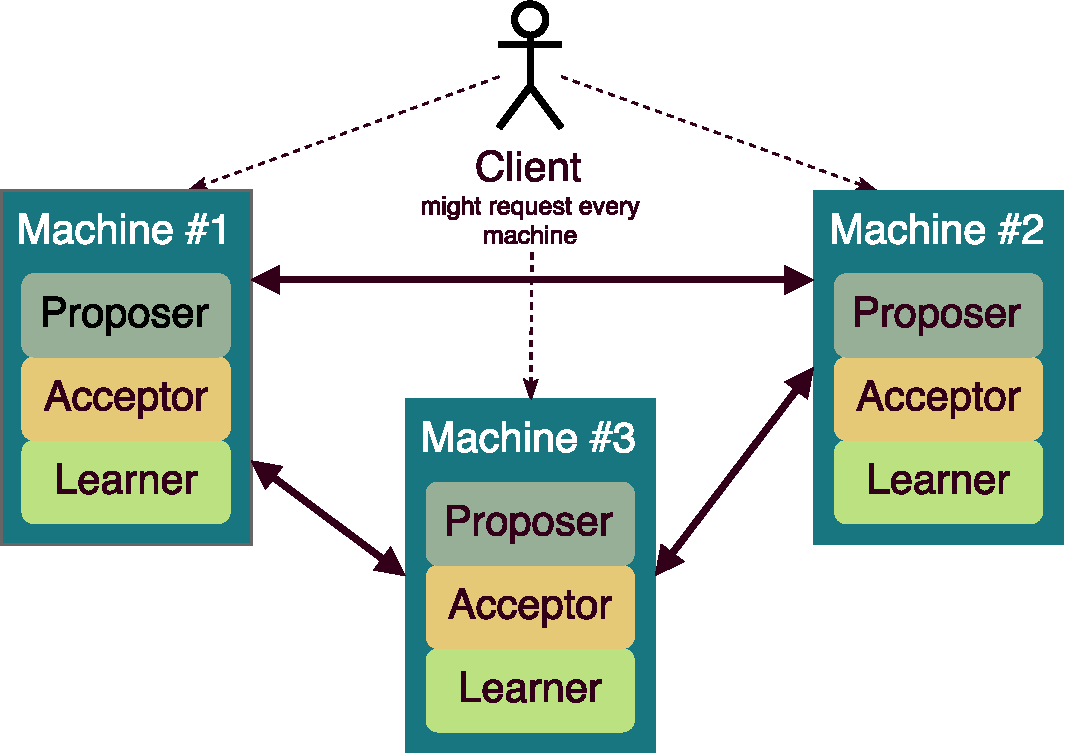
\includegraphics[width=0.8\textwidth]{fig/PaxosSetup.pdf}
	\caption{Example Setup of Three Machines Agreeing on Values Based on the Paxos Algorithm}
	\label{fig:paxosSetup}
\end{figure}

\begin{table}[ht]
    \centering
    \begin{tabularx}{\linewidth}{@{}>{\bfseries}l@{\hspace{.5em}}X@{}}
        \toprule
        \textbf{Operation related to data item} & \textbf{Consequence for vector of data item}\\ \midrule
        Update on site $S_i$ & Increment $v_i$ by one\\
        Delete or rename on site $S_i$ & Keep vector and increment $v_i$ by one, remove data item value\\
        Reconcile version conflict & Set each $v_i$ to maximum $v_i$ from all vectors used for reconciliation. In addition, increment $v_i$ of site that initiated reconciliation by one\\
        Copy to new site & Augment vector to include new site\\
        \bottomrule
    \end{tabularx}
    \caption{Influence of Operations on a Data Item's Version Vector}
    \label{tab:vectorOperations}
\end{table}

Thus, many executives feel fear to become unconscious 
Also, I want to buy \signal{smart home devices} such as the ones listed in table \ref{tab:scenario1_sensor}.

\LTXtable{\textwidth}{tab/scenario1_sensor}

\begin{cEnum}
    \item Analysis ...
    \item Design ...
    \item Prototypical implementation of the design.
\end{cEnum}

The \textbf{client}